\documentclass[twoside,12pt,a4paper,notitlepage]{memoir}

\usepackage{xltxtra,fontspec,xunicode}
\defaultfontfeatures{Scale=MatchLowercase}
\setmainfont{CMU Sans Serif}

\usepackage[top=1.8cm,bottom=1.8cm,outer=1.8cm,inner=4.2cm]{geometry}

\usepackage{hyperref}
\hypersetup{
    colorlinks=true,       % false: boxed links; true: colored links
    linkcolor=black,          % color of internal links (change box color with linkbordercolor)
    citecolor=black,        % color of links to bibliography
    filecolor=blue,      % color of file links
    urlcolor=blue           % color of external links
}

%\usepackage{rotating}
\usepackage{pdfpages}
\usepackage[none]{hyphenat}
\usepackage{lipsum}

\usepackage{graphicx}
\usepackage{wrapfig}

\makeatletter
\let\l@chapternonum\l@chapter
\newcounter{chapternonum}
\renewcommand{\thechapternonum}{}
\makeatother



\begin{document}
\pagestyle{plain}

% Poster
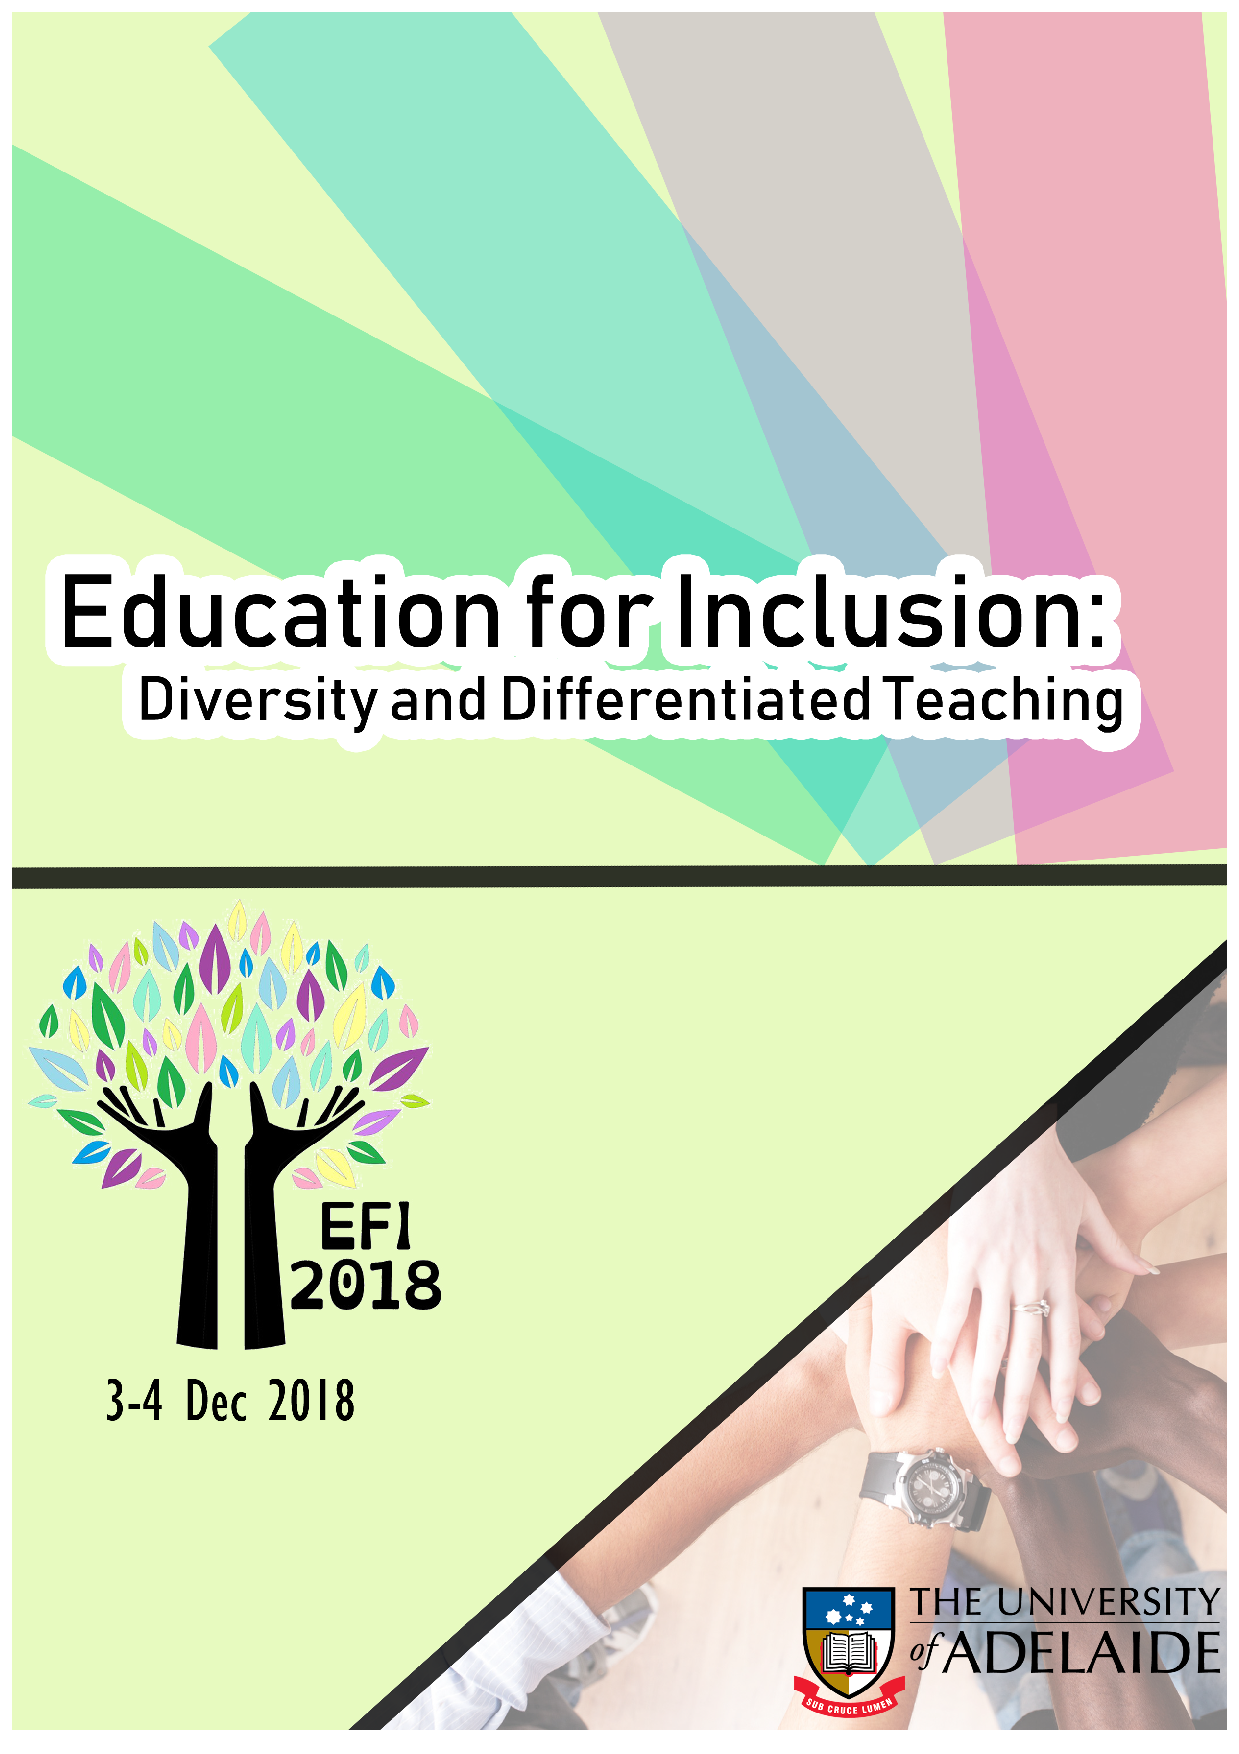
\includepdf[page = 1]{poster.pdf}

% Contents
\setcounter{tocdepth}{2}
\tableofcontents
\vfill

% Acknowledgement of Country
\clearpage\phantomsection
\vspace*{2cm}
{\Huge Acknowledgement of Country}
\vspace{2cm}
\addcontentsline{toc}{chapter}{Acknowledgement of Country}

We acknowledge and pay our respects to the Kaurna people, the traditional custodians whose ancestral lands we gather on. We acknowledge the deep feelings of attachment and relationship of the Kaurna people to country and we respect and value their past, present and ongoing connection to the land and cultural beliefs.
\vfill

\clearpage\phantomsection
% About the Conference
\vspace*{2cm}
{\Huge About the Conference}
\vspace{2cm}
\addcontentsline{toc}{chapter}{About the Conference}

This conference is organised by preservice teachers currently studing a Masters of Teaching at the University of Adelaide and currently enrolled in the course ``Education for Inclusion'. These preservice teachers will also be the presenters for the conference. Presentations will cover a range of issues and interests across multiple disciplines, but centred around inclusive secondary education with a focus on students with disabilities and students from diverse cultural backgrounds, particularly Indigenous students. The intent of this conference is to inform teachers of some of the rewards, difficulties and strategies to effectively teach inclusively. 
\vfill



% Program

\clearpage\phantomsection
\vspace*{2cm}
{\Huge Program}
\vspace{2cm}
\addcontentsline{toc}{chapter}{Program}

\begin{itemize}
	\item The abbreviation `BSS' refers to the Barr Smith South Building (See H11 on the map below).
	\item Flentje Lecture Theatre can be found on level 2-3 of BSS.
	\item Presenter's names are hyperlinked to their abstracts and bios.
	\item Presentation titles are shown in expanded programs for each session.
\end{itemize}

\renewcommand{\arraystretch}{1.4}
%\begin{sidewaystable}
\begin{center}
\begin{tabular}{rcr|p{3.6cm}|p{3.6cm}|p{3.6cm}}
\multicolumn{6}{c}{{\large MONDAY 3 December 2018}} \\ \hline
8.30 & - & 9.00 & \multicolumn{3}{l}{Registration (Flentje Lecture Theatre)} \\ \hline
9.00 & - & 9.10 & \multicolumn{3}{l}{Welcome to Country: Uncle Rod O'Brien} \\ \hline
9.10 & - & 10.00 & \multicolumn{3}{l}{Keynote Speaker: Betty-Jean Price} \\ \hline
10.00 & - & 10.30 & \multicolumn{3}{l}{Morning Tea (BSS 1063)} \\ \hline
 & & & A-Stream \hspace{1cm} (BSS 1062) & B-Stream \hspace{1cm} (BSS 1063) & C-Stream \hspace{1cm} (BSS 2051) \\ \hline
 10.30 & - & 10.55 & 
 \hyperref[aut:winderbaum]{Lyron Winderbaum} & 
 \hyperref[aut:hu]{Di Hu} &  
 \hyperref[aut:atkins]{Natasha Atkins} \\ \hline
11.00 & - & 11.25 &
 \hyperref[aut:anderson]{Craig Anderson} &
 \hyperref[aut:hoskin]{Elliot Hoskin} &
 \hyperref[aut:hanley]{Jacob Hanley} \\ \hline
11.30 & - & 11.55 &
 \hyperref[aut:tymukas]{Benjamin Tymukas} &
 \hyperref[aut:demasi]{Eliza Demasi} &
 \hyperref[aut:hua]{Vinh-Huy `Felix' Hua}  \\ \hline
12.00 & - & 12.25 &
\hyperref[aut:crowhurst]{Nick Crowhurst} &
 \hyperref[aut:west]{Tory West} &
 \hyperref[aut:boskovic]{Beti Boskovic} \\ \hline
12.30 & - & 1.25 & \multicolumn{3}{l}{Lunch (BSS 1063)} \\ \hline
1.30 & - & 1.55 &
 \hyperref[aut:lewis]{Hannah Lewis} &
 \hyperref[aut:wright]{Nicola Wright} &
 \\ \hline
2.00 & - & 2.25 &
 \hyperref[aut:white]{Joshua White} &
 \hyperref[aut:bonner]{Edward Bonner} &
 \\ \hline
2.30 & - & 2.55 &
 \hyperref[aut:barritt]{Betula Barritt} &
 \hyperref[aut:hodkinson]{Lewis Hodkinson} &
 \\ \hline
\end{tabular}
\end{center}
%\end{sidewaystable}
\vfill


\pagebreak
\begin{center}
\begin{tabular}{rcr|p{10.8cm}}
 \multicolumn{4}{c}{{\large A-Stream (BSS 1062) --- MONDAY 3 December 2018}} \\ \hline
 10.30 & - & 10.55 & 
 \hyperref[aut:winderbaum]{The Importance of Cultural and Linguistic Context when Learning Mathematics. (Lyron Winderbaum)} \\ \hline
11.00 & - & 11.25 &
 \hyperref[aut:anderson]{Effective Indigenisation of Middle School Mathematics While Negating Tokenism, Counteracting Anxiety, and Eliminating Prejudice (Craig Anderson)} \\ \hline
11.30 & - & 11.55 &
 \hyperref[aut:tymukas]{Harnessing Language in Indigenous Education (Benjamin Tymukas)} \\ \hline
12.00 & - & 12.25 &
 \hyperref[aut:crowhurst]{Education in Remote Areas: Analysing the Level of Schooling Available in Remote Australia and the Viability of Students from These Areas Accessing Metropolitan Schooling. (Nick Crowhurst)}  \\ \hline
12.30 & - & 1.25 & Lunch (BSS 1063) \\ \hline
1.30 & - & 1.55 &
 \hyperref[aut:lewis]{Twice Exceptional Students with a Visual Impairment: Implications for the Secondary Music Classroom (Hannah Lewis)} \\ \hline
2.00 & - & 2.25 &
 \hyperref[aut:white]{Improving Indigenous Engagement and Development in Mathematics (Joshua White)} \\ \hline
2.30 & - & 2.55 &
 \hyperref[aut:barritt]{Teaching Indigenous Content Respectfully, Sensitively and Confidently in Classroom Music (Betula Barritt)} \\ \hline
\end{tabular}
\end{center}

\begin{center}
\begin{tabular}{rcr|p{10.8cm}}
\multicolumn{4}{c}{{\large B-Stream (BSS 1063) --- MONDAY 3 December 2018}} \\ \hline
 10.30 & - & 10.55 & 
\ \hyperref[aut:hu]{Mental Disorders in Children and the Role of Schools/Teachers (Di Hu)} \\ \hline
11.00 & - & 11.25 &
 \hyperref[aut:hoskin]{Incorporating Culturallly Responsive Pedagogies in English Units: Anh Do's The Happiest Refugee (Elliot Hoskin)} \\ \hline
11.30 & - & 11.55 &
 \hyperref[aut:demasi]{Supporting International Students in Mainstream School Settings: Insights and Strategies for Teachers. (Eliza Demasi)} \\ \hline
12.00 & - & 12.25 &
 \hyperref[aut:west]{Students with Refugee Experience in the Science Classroom: Challenges Faced and Implications for Teachers (Tory West)} \\ \hline
12.30 & - & 1.25 & Lunch (BSS 1063) \\ \hline
1.30 & - & 1.55 &
 \hyperref[aut:wright]{Integrating Parental Involvement to Support Students with a Disability in the Secondary Education Environment (Nicola Wright)} \\ \hline
2.00 & - & 2.25 &
 \hyperref[aut:bonner]{A Guide to Negotiated Education Plans for Preservice and New Teachers (Edward Bonner)} \\ \hline
2.30 & - & 2.55 &
 \hyperref[aut:hodkinson]{No Title Submitted (Lewis Hodkinson)} \\ \hline
\end{tabular}
\end{center}

\pagebreak
\vspace*{0cm}
\begin{center}
\begin{tabular}{rcr|p{10.8cm}}
 \multicolumn{4}{c}{{\large C-Stream (BSS 2051) --- MONDAY 3 December 2018}} \\ \hline
 10.30 & - & 10.55 & 
 \hyperref[aut:atkins]{Attention Deficit Hyperactivity Disorder (ADHD) in a Secondary Classroom (Natasha Atkins)} \\ \hline
11.00 & - & 11.25 &
 \hyperref[aut:hanley]{Understanding and Supporting Auditory Processing Disorders in the Classroom (Jacob Hanley)} \\ \hline
11.30 & - & 11.55 &
\hyperref[aut:hua]{The Inclusion of Students of Attention Deficit Hyperactivity Disorder (ADHD) in the Classroom Context (Vinh-Huy `Felix' Hua)} \\ \hline
12.00 & - & 12.25 &
 \hyperref[aut:boskovic]{Strategies for Teaching Foreign Languages to Students with Dyslexia (Beti Boskovic)} \\ \hline
12.30 & - & 1.25 & Lunch (BSS 1063) \\ \hline
1.30 & - & 1.55 &
 \\ \hline
2.00 & - & 2.25 &
 \\ \hline
2.30 & - & 2.55 &
 \\ \hline
\end{tabular}
\end{center}


\pagebreak
\vspace*{0cm}
\begin{center}
\begin{tabular}{rcr|p{3.6cm}|p{3.6cm}}
\multicolumn{5}{c}{{\large TUESDAY 4 December 2018}} \\ \hline
8.30 & - & 9.00 & \multicolumn{2}{l}{Registration (Flentje Lecture Theatre)} \\ \hline
 & & & D-Stream \hspace{1cm} (BSS 1062) & E-Stream \hspace{1cm} (BSS 1063) \\ \hline
9.00 & - & 9.25 &
 \hyperref[aut:huxtable]{Joshua Huxtable} &
\hyperref[aut:panozzo]{James Panozzo} \\ \hline
9.30 & – & 9.55 &
 \hyperref[aut:bailey]{Matthew Bailey} &
 \hyperref[aut:vogel]{Christopher `Kit' Vogel}  \\ \hline
10.00 & – & 10.25 &
 \hyperref[aut:button]{Robert Button} &
\hyperref[aut:sun]{Ting Sun} \\ \hline
10.30 & – & 10.55 & \multicolumn{2}{l}{Morning Tea (BSS 1063)} \\ \hline
11.00 & – & 11.25 & 
\hyperref[aut:suh]{Kyuseop `Anton' Suh} &
 \hyperref[aut:markovic]{Elda Markovic} \\ \hline
11.30 & – & 11.55 &
 \hyperref[aut:riehl]{Dhani Riehl} &
 \hyperref[aut:johnson]{Patrick Johnson} \\ \hline
12.00 & – & 12.25 &
 \hyperref[aut:ruthven]{Hayley Ruthven} &
 \hyperref[aut:daughtry]{Jonathan Daughtry} \\ \hline
12.30 & – & 1.25 & \multicolumn{2}{l}{Lunch (BSS 1063)} \\ \hline
1.30 & – & 1.55 &
 \hyperref[aut:yan]{Siqin Yan} &
 \hyperref[aut:huang]{Yilun Huang} \\ \hline
2.00 & – & 2.25 & 
 \hyperref[aut:brown]{Hannah Martin-Brown} &
 \hyperref[aut:heath]{David Heath} \\ \hline
2.30 & – & 3.00 & \multicolumn{2}{l}{Closing Address: Michael Colbung (Flentje Lecture Theatre)} \\ \hline
\end{tabular}
\end{center}


\pagebreak
\begin{center}
\begin{tabular}{rcr|p{10.8cm}}
 \multicolumn{4}{c}{{\large D-Stream (BSS 1062) --- TUESDAY 4 December 2018}} \\ \hline
9.00 & - & 9.25 &
 \hyperref[aut:huxtable]{Catering for Blind and Visually Impaired Students in a Music Class Room (Josh Huxtable)} \\ \hline
9.30 & – & 9.55 &
 \hyperref[aut:bailey]{Supporting Students with Autism Spectrum Disorder in a Secondary Music Classroom (Matthew Bailey)} \\ \hline
10.00 & – & 10.25 &
 \hyperref[aut:button]{The Importance of Teachers Being Prepared to Teach Students with a Disability
 (Robert Button)} \\ \hline
10.30 & - & 10.55 & Morning Tea (BSS 1063) \\ \hline
11.00 & – & 11.25 & 
\hyperref[aut:suh]{Numerous Problems: Inclusion of Students with Dyscalcula in Secondary STEM Education (Kyuseop `Anton' Suh)} \\ \hline
11.30 & – & 11.55 &
 \hyperref[aut:riehl]{Improving the Scientific Literacy Skills of Adolescents with Autism Spectrum Disorder in Secondary Classrooms (Dhani Riehl)} \\ \hline
12.00 & – & 12.25 &
 \hyperref[aut:ruthven]{Comparing Programs for Indigenous Students in Australia and Canada (Hayley Beth Ruthven)} \\ \hline
12.30 & - & 1.25 & Lunch (BSS 1063) \\ \hline
1.30 & – & 1.55 &
 \hyperref[aut:yan]{No Title Submitted (Siqin Yan)} \\ \hline
2.00 & – & 2.25 & 
 \hyperref[aut:brown]{Dyslexia; Small Things to Help a Big Problem. (Hannah Martin-Brown)} \\ \hline
\end{tabular}
\end{center}

\begin{center}
\begin{tabular}{rcr|p{10.8cm}}
 \multicolumn{4}{c}{{\large E-Stream (BSS 1063) --- TUESDAY 4 December 2018}} \\ \hline
9.00 & - & 9.25 &
 \hyperref[aut:panozzo]{Effect of Streaming on the Academic and Social Development of Students with Learning Disabilities (James Panozzo)} \\ \hline
9.30 & – & 9.55 &
\hyperref[aut:vogel]{Closing the Other Gap: Boys in Education (Christopher `Kit' Vogel)} \\ \hline
10.00 & – & 10.25 &
\hyperref[aut:sun]{Assisting Hearing Impaired Students Within the Classroom (Ting Sun)} \\ \hline
10.30 & - & 10.55 & Morning Tea (BSS 1063) \\ \hline
11.00 & – & 11.25 & 
 \hyperref[aut:markovic]{Inclusion of Students with Disabilities in High School Chemistry Laboratories (Elda Markovic)} \\ \hline
11.30 & – & 11.55 &
 \hyperref[aut:johnson]{Fostering Inclusivity in Education for Teenage Parents (Patrick Johnson)} \\ \hline
12.00 & – & 12.25 &
 \hyperref[aut:daughtry]{Autism Spectrum Disorder (Jonathan Daughtry)} \\ \hline
12.30 & - & 1.25 & Lunch (BSS 1063) \\ \hline
1.30 & – & 1.55 &
 \hyperref[aut:huang]{An Analysis of Errors and Strategies in the Expository Writing of Students with Learning Disablilities (Yilun Huang)} \\ \hline
2.00 & – & 2.25 & 
 \hyperref[aut:heath]{Empowering Students with Attention Deficit Hyper-Activity Disorder (ADHD) (David Heath)} \\ \hline
\end{tabular}
\end{center}




\clearpage\phantomsection
\includepdf[pages = 3]{map.pdf}
\addcontentsline{toc}{chapter}{Map}


% Keynote Speakers.
\clearpage\phantomsection
\vspace*{2cm}
{\Huge Invited Speakers}
\vspace{2cm}
\addcontentsline{toc}{chapter}{Invited Speakers}

\section*{Dr Betty-Jean Price}
\addcontentsline{toc}{section}{Dr Betty-Jean Price}

\begin{wrapfigure}{R}{0.4\textwidth}
\centering
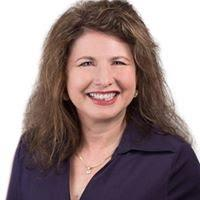
\includegraphics[width=0.35\textwidth]{betty_jean.jpg}
\end{wrapfigure}

Dr Betty-Jean (B-J) Price has a background in education and social work, is a progressive and experienced manager, community leader, sessional lecturer and tutor in social work education.  Since the late 1990’s, B-J has participated on equity-centred committees such as the SA Drug Court Treatment Committee, SACOSS Law and Justice Committee, Mental Health Magistrates Court (Managers Committee) and the Adelaide City Council Access and Inclusion Panel.  Prior to this, B-J practised social work in a variety of roles including a Professional Services Officer (PSO3) role in community health, as well as the management of drug treatment services for offenders in correctional settings. In 2013 B-J was awarded a full PhD scholarship from the Southgate Institute for Health Society and Equity; this furthered her interests in disability, particularly in the area of complex communication needs, and disability-friendly research methodology. Having completed her thesis, B-J is a passionate campaigner for human rights, inclusive education and disability health policy. Earlier this year, B-J was employed by the Department of the Premier and Cabinet to write disability, inclusive education and mental health policy.  B-J is a published author, national and international conference presenter, and an active research partner with Cerebral Palsy Research Alliance and Sydney University.  B-J’s current committee participation includes the Australasian Association of Cerebral Palsy and Developmental Medicine and the Cerebral Palsy Alliance Stem Cell Research Reference Group.
\vfill


\clearpage\phantomsection
\vspace*{2cm}
\section*{Michael Cobung}
\addcontentsline{toc}{section}{Michael Cobung}

\begin{wrapfigure}{R}{0.4\textwidth}
\centering
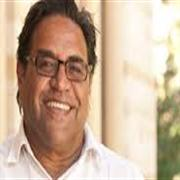
\includegraphics[width=0.35\textwidth]{michael_colbung.jpeg}
\end{wrapfigure}

Michael Colbung is a lecturer and researcher with the School of Education at the University of Adelaide in the Faculty of Arts. 

He currently teaches a fourth year subject, “Education, Culture and Diversity”, and a Master’s course, “Education for Inclusion”. In these courses he is able to give a firsthand account of Aboriginal and Islander peoples negotiating a western educational system as he is a Wongatha (Wongi) / Nyoongah man with strong cultural links to the Wirangu and Kookatha nations.

His research has allowed him to work on a number of projects in Aboriginal communities and attach the necessary sensitivities when undertaking research with Aboriginal families and their communities.

He is a qualified teacher, having taught in a variety of teaching positions and an expert at creating a classroom that is flexible and suits a diverse range of learners.
\vfill


\clearpage\phantomsection
\vspace*{2cm}
\section*{Uncle Rod O'Brien}
\addcontentsline{toc}{section}{Uncle Rod O'Brien}

\begin{wrapfigure}{R}{0.4\textwidth}
\centering
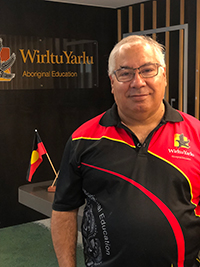
\includegraphics[width=0.35\textwidth]{Uncle_Rod.jpg}
\end{wrapfigure}

From \href{https://www.adelaide.edu.au/wirltu-yarlu/cultural-advisors/}{the Wirltu Yarlu Cultural Advisors page on the University of Adelaide website}:

Rod identifies as a Kaurna man and devotes much time to helping other Kaurna people identify with the language and culture. He is an active member of the Adelaide Aboriginal community, volunteering his time as a Chairperson on a number of committees which include the Kaurna Warra Karrpanthi Aboriginal Corporation, Kaurna Yerta Aboriginal Corporation and Kura Yerlo Inc.

Rod has an Honours and Bachelor's Degree in Applied Science in Aboriginal Community Development and Management from Curtin University. Prior to joining Wirltu Yarlu, he worked in the State Government for over 23 years in the Department for Child Protection.

Rod is passionate about reclaiming Kaurna language, and hopes to see Kaurna language and culture being in taught in every school in the Adelaide Plains region.

"My dream is for the Kaurna language to be revived to a level where there are hundreds of people able to converse in it with meaningful dialogue on a daily basis. For I believe, if it is spoken, people will gain strength, knowledge and power from its us, thus keeping alive Kaurna culture."



% Preservice Teacher Presentations
\clearpage\phantomsection
\vspace*{2cm}
{\Huge Preservice Teacher Presentations}
\vspace{2cm}
\addcontentsline{toc}{chapter}{Preservice Teacher Presentations}


\section*{Effective Indigenisation of Middle School Mathematics While Negating Tokenism, Counteracting Anxiety, and Eliminating Prejudice (Craig Anderson)}
\addcontentsline{toc}{section}{Effective Indigenisation of Middle School Mathematics While Negating Tokenism, Counteracting Anxiety, and Eliminating Prejudice (Craig Anderson)}
\label{aut:anderson}

In the decade after 2006, Australian school students’ performance rankings - mathematics in particular - have dropped in relation to other OECD nations. Furthermore, in accordance with the 2017 SACE enrolment records, much to the discontent of Australian Chief Scientist Alan Finkel, the enrolments in specialist mathematics was significantly lower than the enrolments in physics and chemistry; subjects where specialist mathematics is required at the university level.

It is evident that modern day school students walk a fine line between success and failure within mathematics. The addition of ‘irrelevant’ - or tokenistic - content to an already declining subject does little to alleviate anxiety amongst students. Furthermore, one might argue that tokenism in fact increases prejudice to an already poorly represented culture.
More alarmingly, the prejudice exists at the federal level as seen with the 2018 federal Liberal leader candidate Peter Dutton, and former Liberal shadow minister Sophie Mirabella boycotting the 2008 Rudd Sorry Speech. Furthermore, such recalcitrant views are further compounded by former prime minister - and at the time leader of the opposition - Tony Abbott’s insensitive comments about the Aboriginal Tent Embassy in Canberra. It seems farcical to imagine that any positive change could occur with xenophobic legislators.
In a modern era, this presentation explores 1) the nexus between mathematics and culture, 2) the relevance of indigenous content within mathematics, and 3) the usage of culture to counteract anxiety within mathematics. By the end of this presentation, the goal is to commence a pragmatic dialogue on how to equip students with the necessary skills to operate both intelligently and compassionately in an ever-changing technology era.

\section*{Craig Anderson}

Craig completed a Bachelor of Engineering, Computer Engineering, Honors Class II Division 1 from University of Wollongong in June of 2012.

Afterwards, Craig moved to Melbourne where he worked as an engineer specialising in electronics circuit design, embedded firmware development, production, and equipment service \& repair. Craig ultimately left engineering in pursuit of a more ‘human’ work environment.

Craig is currently studying a Master of Teaching at University of Adelaide, with the intention of bringing exciting industrial applications to the classroom.

In his spare time, Craig can be found tinkering with his robots, and loitering at cafés.


\pagebreak
\section*{Attention Deficit Hyperactivity Disorder (ADHD) in a Secondary Classroom (Natasha Atkins)}
\addcontentsline{toc}{section}{Attention Deficit Hyperactivity Disorder (ADHD) in a Secondary Classroom (Natasha Atkins)}
\label{aut:atkins}

The Australian Guidelines on Attention Deficit Hyperactivity Disorder (ADHD) (2009) state that 5-10\% of children and adolescents are diagnosed with ADHD, yet throughout education there seems to be a lack of well-known and easily employable strategies to aid these students at a secondary level. It is recognised that students with ADHD often experience social and academic problems in the classroom (Lessing \& Wulfsohn, 2015) and this research aims to explore and expand on common strategies that are more prominent in primary classrooms and adapt them for use in a secondary space.


ADHD, previously known as Attention Deficit Disorder (ADD) is a neurodevelopmental disorder with a recognised and persistent pattern of behaviour. ADHD begins at birth, for both sexes, and will usually continue through all of life to some degree. ADHD is generally divided into three subcategories: inattentive, hyperactive/impulsive and combined. There is a very large range of symptoms that students with ADHD can show. Typically, students might be easily distracted, forgetful, disruptive and participate in risky, impulsive activities (ADHD Australia), however, educators should realise that the symptoms that each student will display will be different.


DuPaul et al. (2011) suggests a range of strategies to support students with ADHD to overcome their academic difficulties. Some of these strategies include modifying the length or content of assessments, providing students with a choice when asked to complete a task, increasing the use of positive reinforcement and providing more detailed instruction.


It is also important to recognise that students with ADHD can be creative, good public speakers, energetic and enthusiastic (DfE, 2018). Teachers should use each student’s strengths in the classroom to support and encourage their successes. Students with ADHD often have lowered self-esteem because they feel as though they need to work much harder than their peers to complete the same tasks. By incorporating strategies to recognise the positive behaviour of these students, teachers can help lift student’s self-esteem (Child Mind Institute).


Educators need to be aware of a broad range of strategies to incorporate into their secondary planning, lessons and assessments to not only help students with ADHD overcome their difficulties in the classroom, but also to help them flourish by encouraging the use of their strengths, all while maintaining student self-esteem and inclusion.

\section*{Natasha Atkins}

In 2013 Natasha began her tertiary education at the University of Adelaide in a Bachelor of Science (Advanced) which she graduated from in 2015 with a double major in Theoretical and Experimental Physics. In 2016 she began her Master in Astrophysics and graduated from this in 2018 as well as beginning her journey in Master of Teaching.



\pagebreak
\section*{Supporting Students with Autism Spectrum Disorder in a Secondary Music Classroom (Matthew Bailey)}
\addcontentsline{toc}{section}{Supporting Students with Autism Spectrum Disorder in a Secondary Music Classroom (Matthew Bailey)}
\label{aut:bailey}

Within a secondary music classroom, students with Autism Spectrum Disorder (ASD) are at educational risk as a result of not having the necessary support systems in place to meet their needs and requirements. Within ASD, there is a wide range of difficulties that people on the spectrum may face, ranging from high functioning autism (Asperger’s) to nonverbal autism. All people with autism fit on this spectrum differently, thus it is imperative for schools to be able to accommodate both ends of the spectrum. This will be examined through how the Australian Curriculum (ACARA) and South Australian Certificate of Education (SACE) meet the legislative requirements necessary to support these students within a mainstream music classroom. Within this, the curriculum documents will be investigated to determine if there is enough alteration of curricula to provide adequate support for ASD students, particularly focusing on providing opportunities for active participation.


From a legislative standpoint, several documents such as the Disability Discrimination Act (1992) and the subsequent Disability Standards for Education (2005) have been written to support these students. These legislative documents have been examined to identify the scope of support that students with ASD are entitled to in relation to the curricula. In addition, documents such as the Department for Education and Child Development’s ‘Children and Young People Disability Policy’ have been written and appraised, which divides the roles and responsibilities in providing an inclusive education for various levels of authority (e.g. Chief Executive, Teachers, Principals, School Services Officers).


These support systems and legislations require constant communication between schools and parents/carers so that the most effective methods of giving the student an inclusive education are considered. Some of the current methodologies in place include Individual Learning Plans (ILP) and Negotiated Education Plans (NEP), which classroom teachers design in consultation with the parents/carers and school to give their student the necessary support and resources for their education.

The findings of this conference will provide secondary music teachers with strategies to help implement a classroom environment which is inclusive to students with ASD. These strategies will be tailored in accordance with legislative documents and requirements, as well as the SACE and ACARA curriculum documents, whilst also having a focus on the support systems in place which can aid students and teachers with this inclusive method of education.

\section*{Matthew Bailey}

Matthew has completed a Bachelor of Music from the Elder Conservatorium of Music, specialising in Jazz Performance. Since then, he has moved into the Master of Teaching program, specialising in Classroom and Instrumental Music.


\pagebreak
\section*{Teaching Indigenous Content Respectfully, Sensitively and Confidently in Classroom Music (Betula Barritt)}
\addcontentsline{toc}{section}{Teaching Indigenous Content Respectfully, Sensitively and Confidently in Classroom Music (Betula Barritt)}
\label{aut:barritt}

Within the Australian Curriculum and the South Australian Certificate of Education (SACE), there resides a strong emphasis on the inclusion of Aboriginal and Torres Strait Islander content across all learning areas. However, to many music educators, teaching Aboriginal and Torres Strait Islander content can prove a daunting task and many non-Indigenous teachers avoid teaching this topic completely. The issue arises when teachers who have little to no knowledge of the topic are expected to teach it at a proficient level, often without opportunities to develop cultural competency (Booth, 2014). Therefore, music educators often feel overwhelmed due to the complex issues surrounding race, history and politics that surface when teaching this content (Mackinlay, 2008).


So, due to the complex barriers of history, politics and race, how can music educators equip themselves with the tools and knowledge to sensitively, respectfully and confidently teach the music and culture of Aboriginal and Torres Strait Islander peoples with the overall goal of working towards reconciliation and intercultural inclusiveness?


This presentation aims to explore some of the practical strategies that all secondary music teachers can use in their classrooms to teach Indigenous music and culture with confidence and respect. Primary among these strategies will be the ideas presented by Elizabeth Mackinlay in her article, ‘Making Space as White Music Educators for Indigenous Australian Holders of Song, Dance and Performance Knowledge: the Centrality of Relationship as Pedagogy (2008)’. In this article, Mackinlay discusses a different perspective of the use of relationships when teaching Indigenous music and culture in the classroom, which goes outside the box of teacher-student, student-student relationships, and into the relationship we have with the country we teach on.


\section*{Betula Barritt}

Betula has completed a Bachelor of Music (Majoring in Classical Performance) at the Elder Conservatorium of Music. She is a Private Music Instructor on the flute and recorder and has been teaching instrumental music for the past eight years. She looks forward to working in a classroom music setting as well as broadening her experiences as an instrumental teacher through the Master of Teaching Degree. She has a passion for inclusive teaching and seeks to continue researching and participating in this field.



\pagebreak
\section*{A Guide to Negotiated Education Plans for Preservice and New Teachers (Edward Bonner)}
\addcontentsline{toc}{section}{A Guide to Negotiated Education Plans for Preservice and New Teachers (Edward Bonner)}
\label{aut:bonner}

For almost two decades in South Australia, schools have been constructing and employing personalised education plans for students with disabilities. This presentation aims to create a level of understanding about how personalised education plans work and to dispel confusion surrounding the topic to give preservice teachers and new teachers the information necessary to confidently aid in the construction of a personalised education plan. 


The department strives to provide learning programs that meet the needs and requirements of all students as well as complying with the Early Years Learning framework and the Australian Curriculum. Furthermore, all schooling authorities are aware of their responsibility to provide “equality before the law in the area of education” for students with disabilities. 


These personalised education plans are known as Negotiated Education Plans (NEPs) and are ubiquitous in high schools. Despite their prevalence in South Australian schools, they can be difficult to interpret, understand and implement for student teachers and teachers that are newly graduated. Each school may have its own unique structure to NEP paperwork which adds to the confusion. There are strict guidelines that govern NEPs to ensure that care is taken in their construction, implementation and continued compilation over the learner’s educational life. The NEP provides a foundation for decision making that is based on the clear and shared understanding of the NEP student’s strengths, interests and needs as well as how the learner best learns. Overall, the NEP is a tool to minimise or mitigate barriers to learning to promote success for students with a disability.

\section*{Edward Bonner}

Edward has a degree in Marine Biology and is undertaking a Master of Teaching at the University of Adelaide. Labelled as non-academic in his formative years, he left school early, resenting the experience. Thereafter he completed an electrical apprenticeship and worked in mining across Australia. A desire and passion for learning brought him to tertiary education. Unwilling to let students fall through the cracks and be forgotten, Edward seeks to make a positive impact on every student in his class.



\pagebreak
\section*{Strategies for Teaching Foreign Languages to Students with Dyslexia (Beti Boskovic)}
\addcontentsline{toc}{section}{Strategies for Teaching Foreign Languages to Students with Dyslexia (Beti Boskovic)}
\label{aut:boskovic}

Dyslexia denotes specific difficulties in word decoding and encoding, which reflects in children facing challenges in reading, spelling and consequently, writing. It used to be easy to refer to dyslexic students as ‘poor readers’, and put the developmental cognitive disorder aside due to an ignorance or a lack of knowledge about the learning difficulty. Nowadays, more and more studies are being done regarding the issue, furthermore, strategies are being developed that can be directly applied in a classroom. However, interdisciplinary research is of utter importance as the phenomenon in question is multi-layered and needs to be tackled on multiple levels, e.g. genetics, linguistics, pedagogy, neurobiology as well as through cognitive psychology and socio-cultural or socio-economic studies. 


The primary aim of this research was to gather information about dyslexia and dyslexic students that would be relevant to teachers of foreign languages and would provide them with some practical teaching methods which they can employ in a language classroom. Many learning disabilities researches suggest that foreign language learning is greatly based on language skills in the student’s first language. Therefore, dyslexia complicates learning of a foreign language in the core. The metalinguistic knowledge helps dyslexic students with terminology when learning a new language, with organizing and making sense of the sentence and grammatical structures, as well as with recognizing and applying the language patterns. Researches included in this paper are mainly based on theories about dyslexia and practical case studies of dyslexic students and/or authors’ own experiences with the foreign language learning and/or being dyslexic themselves. 



Researchers imply various surviving strategies for dyslexic students of a foreign language, naming perseverance and hard work, finding a hard work-wellbeing balance, using instructors who can help them find patterns in their first language that could aid them in learning the foreign language, preparing for classes by reading a chapter before it is taught in class and accepting the foreign language without debating the logic behind it.

For language teachers the following strategies are pointed out: encouraging students to make charts where they can observe language patterns, singing songs and giving students opportunities to practise memorised dialogues, as well as giving students immediate and transparent feedback.

\section*{Beti Boskovic}

Beti completed a double degree in Comparative Literature and Teaching of Slovenian Language at University of Ljubljana, Slovenia in 2011. In 2012, she did a study exchange in Angers, France within her studies of Interlingual Communication (with two majors being English and French) which she finished in 2018 at University of Ljubljana, Slovenia. Following her passion of teaching languages, she undertook a TESOL course at TAFE, Adelaide in 2016, and is currently finishing a Master Degree at University of Adelaide, specialising in teaching French and EALD.
She worked as a teacher of Slovenian language as a second/foreign language at various institutions, including University of Ljubljana and University of Primorska, in Slovenia for four years, as well as working on various translating projects. Currently, she does tutoring and private lessons for French.
To take a break from various linguistic engagements, Beti loves to cook (and eat), talk to birds while hiking and participate as a passionate rock climber.


\pagebreak
\section*{The Importance of Teachers Being Prepared to Teach Students with a Disability (Robert Button)}
\addcontentsline{toc}{section}{The Importance of Teachers Being Prepared to Teach Students with a Disability (Robert Button)}
\label{aut:button}


It is important to identify productive teaching strategies for students who have a learning disability. There are many different learning disabilities and disorders that secondary school students in Australia live with every day. Disabilities and disorders that are frequently encountered by teachers in classrooms include dyslexia and Attention Deficit Hyperactivity Disorder (ADHD) to name a couple. Every school should strive to be inclusive of students with learning disabilities and much of this inclusivity relies on the teachers in the classroom. It is easy for schools to be labelled as “inclusive”, but this implies that every teacher employed on site has a vast knowledge on how to teach students with a variety of disabilities. Sometimes it is hard for teachers to consider each students’ satisfaction with the classroom environment and there isn’t an easy way to gauge satisfaction levels.

The problem that this research aims to solve is how to successfully teach a range of students with disabilities in mainstream classrooms. The Australian Research Alliance for Children and Youth (ARACY) note that each state and territory currently has different approaches to assessment and reporting for students with a disability, meaning this inconsistency makes it difficult for educational institutions to determine if appropriate progress is being made. ARACY have conducted previous research that focussed on whole school inclusive practice and identified in-class inclusive practice such as quality teaching and alternative curricula.

\section*{Robert Button}

Robert completed a Bachelor of Arts at The University of Adelaide in 2016 with a major in English and minors in History and Anthropology. After taking a short break from studying, he has returned to undertake a Master of Teaching specialising in Senior English and Senior History. He looks forward to the exciting challenges that a career in the teaching profession will present. In his time outside of university commitments, he can be found working at his part-time job in the retail field and is a self-described “film enthusiast.”



\pagebreak
\section*{Education in Remote Areas: Analysing the Level of Schooling Available in Remote Australia and the Viability of Students from These Areas Accessing Metropolitan Schooling. (Nick Crowhurst)}
\addcontentsline{toc}{section}{Education in Remote areas: Analysing the Level of Schooling Available in Remote Australia and the Viability of Students from These Areas Accessing Metropolitan Schooling. (Nick Crowhurst)}
\label{aut:crowhurst}

Australia is renowned as a sparsely populated country, with the majority of its activity being centred around its metropolitan areas. This is reflected in statistics; 71\% of Australian residents are located in major cities while only 2\% live in remote or very remote communities. These numbers, however, do not accurately reflect the distribution of Aboriginal and Torres Strait Islander peoples; 37\% live in major cities while 20\% live in remote or very remote communities.
 
 
This geographic isolation can have a marked impact on the level of formal education students receive. With diminished access to resources, schooling and teachers, students are often left with a limited schooling experience when compared with those in metropolitan areas. Ulterior influences, such as a higher cost of living due to a lack of economies of scale and difficulty in retaining qualified staff, also contribute to a complicated situation where adequate education is not always readily available. These implications are covered in detail through the Education opportunity in Australia 2015 (Lamb, Jackson, Walstab \& Huo) report, detailing the many discrepancies between rural and urban education and further measures that may assist in closing this gap.
 
 
In saying this, such measures, including re-distribution of funding and technological advancement, are often viewed as long-term processes; invaluable for ongoing development but perhaps of little impact to existing students. As such, this presentation aims to also look at the viability of rural students accessing schooling in metropolitan areas where education institutions are statistically more effective. The myriad of factors surrounding the financial and social cost of relocation, methods of doing so and access to government or other assistance will be analysed with a particular emphasis on Aboriginal and Torres Strait Islander peoples given their level of representation in remote or very remote communities.

\section*{Nick Crowhurst}

Nick is undertaking the Master of Teaching program after years studying to enter the corporate world. Majoring in Business and Economics, Nick aims to become a teacher that provides students with a practical real-world skill set to complement curriculum and academic achievement. In his spare time Nick enjoys the outdoors and any beach-related recreational activities. 



\pagebreak
\section*{Autism Spectrum Disorder (Jonathan Daughtry)}
\addcontentsline{toc}{section}{Autism Spectrum Disorder (Jonathan Daughtry)}
\label{aut:daughtry}

ASD is often difficult to identify, and comes with a multitude of challenges. It is vital that educators have a thorough understanding of ASD, and employ strategies for creating inclusive and accommodating environments. The purpose of my presentation is to provide an overview of effective strategies that can assist educators of students with Autism Spectrum Disorder (ASD).
 
My presentation provides an overview of the symptoms of ASD, and explores papers written by leading researchers and academics which uncover strategies that educators can use to improve outcomes for students with ASD. I answer questions such as: How can support networks assist with the success of students with ASD? How can technology be used in order to increase the engagement of secondary students with autism? How can educators modify their learning environments to help students with ASD feel more comfortable?


\section*{Jonathan Daughtry}

Is currently enrolled in the ``Education for Inclusion'' course in the School of Education at the University of Adelaide.



% Strategies to support international students in mainstream Australian classrooms.
\pagebreak
\section*{Supporting International Students in Mainstream School Settings: Insights and Strategies for Teachers (Eliza Demasi)}
\addcontentsline{toc}{section}{Supporting International Students in Mainstream School Settings: Insights and Strategies for Teachers (Eliza Demasi)}
\label{aut:demasi}

In an increasingly competitive and globalised world, many international students are choosing to enrol in Australian schools. By enrolling in both Australian public and independent schools, international students have a better opportunity to enter competitive tertiary education institutions, obtain desirable personal and cultural competencies, and to achieve proficiency in English language. When integrating to Australian schooling systems, international students face a variety of challenges including English-language competency issues, culture shock, homesickness, difficulty adapting to vastly different learning environment norms, and social isolation. International students face not only linguistic barriers in an Australian classroom, but in some cases, must adapt to less teacher-centred, more creative and collaborative learning environments which may contrast to their source country educational systems. Considering the increasing globalisation of the Australian classroom, it is important to identify strategies for teachers to support the inclusion, wellbeing and academic success of this cohort within mainstream classes. 


This presentation aims to outline simple strategies which can be considered for teachers of international students to increase students’ participation, inclusion and success in an Australian classroom setting. It draws on relevant publications and literature, applies theories of EAL pedagogy and examines several everyday examples of inclusive practice from real experiences. It identifies how teachers can better consider the unique needs of international students across multiple subject areas and introduces simple strategies to facilitate improved inclusion for this cohort. Ultimately, the cultural and linguistic strategies for teaching international students can also be adapted to inform improved inclusive teaching practice across a range of student cohorts and subject areas.

\section*{Eliza Demasi}

After completing a Bachelor of Development Studies and a Diploma of Languages (French) in 2014, as well as a Cert. IV in TESOL in 2013, Eliza has returned to study Master of Teaching at the University of Adelaide, specialising in Spanish and English as an Additional Language. Since 2010, she has been teaching community English as an Additional Language (EAL) classes as a volunteer with the Australian Red Cross, as well as teaching business English while on study exchange to Santiago, Chile.

When not getting overexcited about morphemes, Eliza enjoys dance, cooking and literature, and volunteers as a community presenter in the Emergency Services Program with the Australian Red Cross.



% Supporting Students with Auditory Processing Disorders - Classroom Interactions
\pagebreak
\section*{Understanding and Supporting Auditory Processing Disorders in the Classroom (Jacob Hanley)}
\addcontentsline{toc}{section}{Understanding and Supporting Auditory Processing Disorders in the Classroom (Jacob Hanley)}
\label{aut:hanley}

Many educators are provided with substantial resources and training in relation to supporting students with hearing impairment. Approximately one in six Australians have a significant hearing loss, and the impact on student learning is well understood with a range of inclusive teaching strategies available (Australian Disability Clearinghouse on Education and Training, 2018). However, Auditory Processing Disorder (APD) can often be overlooked or symptoms misunderstood as being related to a hearing impairment or other learning disability. Approximately 5\% of school-aged children are affected by APD, and the awareness and support for educators is limited (Morlet, 2014). The focus of this research is to promote awareness of APD, and the relevant strategies that can be implemented in the classroom to increase student engagement and wellbeing.


APD must be treated differently to hearing impairments, as the majority of sufferers will still have normal peripheral hearing. Symptoms of APD include deficits in one or more of the following auditory skill areas; pattern recognition, discrimination, temporal integration and ordering, and dichotic listening (Miller \& Wagstaff, 2011). Diagnosis of APD is also further complicated by the lack of specificity in commercially available tests, resulting in a higher sensitivity to a diverse range of other learning problems. False positive results of APD can be attributed to the acceptance of poor performance on a single modality of testing, without further investigation to other underlying issues (Cacace \& McFarland, 1998). Students diagnosed with APD can exhibit behavior that is often associated with inattentiveness or Attention Deficit Hyperactivity Disorder (ADHD). The student may appear to have missed key parts of instructions, failed to respond to verbal cues, or are unable to discern classroom discussions. This is generally due to aural stimuli being processed at an abnormal rate, or the inability to differentiate mixed sounds and volume levels (Bartlett, Kelley, Purdy, \& Stein, 2017). Symptoms of APD may be heightened in an open or chaotic environment, which often increase the presence of aural stimuli. APD can be supported in the classroom by modifying the environment, amplifying primary audio sources, providing written instructions, and correcting student/teacher spatial positioning. Auditory training combined with repetitive presentation of aural stimuli has also proven to be effective in improving performance on auditory based instructions or tasks (Moore, 2015). These strategies can greatly increase the efficacy of specialist interventions for students with APD, ensuring that the student is supported not only by audiology professionals and psychologists but also by their caretakers and educators.

\section*{Jacob Hanley}

Jacob was awarded a Bachelor of Mechanical Engineering, Honors from Deakin University Geelong in January of 2015.
While completing his degree Jacob worked in nanofiber research, steel fabrication, and welding robotics. Following this, he moved to South Australia to work on various projects including aircraft modification, flight testing, and ERP system implementation. Through his employment, he has been fortunate enough to work briefly in America, Canada, Taiwan and also the Philippines.
At the beginning of 2018, Jacob commenced the Master of Teaching at The University of Adelaide to pursue his passion for education.



% Attention Deficit Hyperactivity Disorder - Empowering Students with ADHD
\pagebreak
\section*{Empowering Students with Attention Deficit Hyperactivity Disorder (ADHD) (David Heath)}
\addcontentsline{toc}{section}{Empowering Students with Attention Deficit Hyperactivity Disorder (ADHD) (David Heath)}
\label{aut:heath}

This research aims to identify the barriers to learning and social development facing students with ADHD and discuss how teachers can empower students with ADHD to manage their disorder to achieve academically.


With the rate of ADHD worldwide at approximately 5.3\% (Polanczyk et al., 2007) Australian teachers must be aware of the disorder and how they may empower students to manage the disorder. The disorder has a broad range of often dichotic symptoms and may manifest in multiple forms. Most symptoms trace back to a student’s struggle to maintain focus on a task or thought process.


The focus of the research was on developing lesson planning suitable to supporting students with ADHD, discussing teaching strategies to support student participation, and closing lessons appropriately (Hallahan, 2009). By demonstrating organisation and self-management strategies to manage classroom process teachers may assist in supplementing the self-regulation of ADHD students. Self-regulation strategies may be developed with students through rapport and a focus on student choice in the creation of their own personal self-regulation strategies. Students must be guided to develop self-reflective processes to empower them to identify choices made and alternate pathways. Empowered students with reinforced self-regulation strategies have been shown to increase on-task behaviour of students with ADHD (Graham-Day \& Gardner, 2010).

\section*{David Heath}

David received his Bachelor of Engineering (Electrical/Electronic - Avionics), Honours, from the University of Adelaide in 2012. David worked as an Engineer within the Defence industry for 5 years prior to returning to study his Master of Teaching at the University of Adelaide majoring in Physics and Senior Mathematics.



\pagebreak
\section*{No Title Submitted (Lewis Hodkinson)}
\addcontentsline{toc}{section}{No Title Submitted (Lewis Hodkinson)}
\label{aut:hodkinson}

No abstract submitted.

\section*{Lewis Hodkinson}

Is currently enrolled in the ``Education for Inclusion'' course in the School of Education at the University of Adelaide.



\pagebreak
\section*{Incorporating Culturally Responsive Pedagogies in English Units: Anh Do's The Happiest Refugee (Elliot Hoskin)}
\addcontentsline{toc}{section}{Incorporating Culturally Responsive Pedagogies in English Units: Anh Do's The Happiest Refugee (Elliot Hoskin)}
\label{aut:hoskin}

As Australia continues to become more multicultural, schools must adapt their curricula so that students from migrant and Aboriginal or Torres Strait Islander backgrounds remain engaged, as well as offering them equal opportunity to reach the outcome of their Anglo-Australian peers. A culturally responsive teacher is aware of both their own cultural capital, as well as the capital that each student brings to class. To be responsive, a teacher must ‘approach… teaching and learning where the educational experiences provided for students should reflect, validate, and promote their culture and language and be cognizant of students’ socio-political histories and future aspirations.’ (Daniels-Mayes 2016: 55) This means that it is a teacher’s role to help their students see their cultural heritage as a benefit, shifting the deficit mindset.


 Krakouer writes, ‘Indigenous students have previously been asked to trade their Aboriginality and cultural beliefs in exchange for a Western education (2016).’ If this is the experience of ATSI students, then it is not difficult to imagine students of a migrant or refugee background would experience a similar cultural jettison to fit within the 
Australian educational system. Culturally responsive teaching aims to render this loss of culture as a thing of the past, as it helps students engage with their culture and use it to benefit their learning.


Over the course of my 45-day placement, I was fortunate enough to be involved in a research project on incorporating culturally responsive pedagogies (CRP) in a Year 10 English class. Along with my mentor teacher, Mrs. Michelle Place, we were able to design and teach a culturally responsive unit on Anh Do’s Novel, \textit{The Happiest Refugee}. The class has 27 students from a variety of cultural backgrounds, including ATSI, Vietnamese, Iraqi, Afghani, Palestinian, Indian, Bangladeshi, Italian as well as Anglo-Celtic. As well as talking about the themes of refugee life in Australia, the unit aimed to encourage students to tell stories from their own families, culminating in a short film task in which students filmed a family member to find out that person’s story. CRP is a growing research area that is relatively new, so this case study is on the cutting edge of determining how to best apply the ideas and practices of CRP.

\section*{Elliot Hoskin}

Elliot has completed a double degree in Media and Arts, as well as a Diploma of English. He comes from a teaching family and wishes to continue setting up adolescents for successful lives. He can’t wait for his Masters to be complete, so he can get out and apply all of this years learning.



\pagebreak
\section*{Mental Disorders in Children and the Role of Schools/Teachers (Di Hu)}
\addcontentsline{toc}{section}{Mental Disorders in Children and the Role of Schools/Teachers (Di Hu)}
\label{aut:hu}

This paper aims to provide a theoretical framework of mental disorders in Australian children and practical solutions that could be implemented by schools/teachers to help these children flourish. According to the Young Minds Matter Mental Health Survey (Lawrence et al., 2015), it was estimated that more than half a million (13.9\%) Australian children aged between 4 and 17 experienced mental disorders during a 12-month survey and around 30\% of these children experienced more than one form of mental disorders. 


The most common mental disorder experienced by these children was ADHD, followed by anxiety disorders while the prevalence varied by gender and age. More than 80\% of these children reported that the mental disorder(s) impacted on their work/school life, family life, friendship, and self-esteem but unfortunately only 17\% of them had used services for support due to various reasons, mostly because of the financial cost of the services and lack of education (Lawrence et al., 2015). With more than 96\% of these children attending schools, schools and teachers play a vital role and can have a positive and significant impact on these children’s’ lives.


There are a number of ways that schools and teachers can support children with mental disorders including education, identification, services at school, and classroom strategies/resources. Public, perceived and self-stigmatising attitudes to mental illness has been identified as the major barrier for help-seeking (Gulliver, Griffiths, \& Christensen, 2010). Schools should integrate mental health education in their curriculum and activities (State Government of Victoria, 2018). In addition, as students spend around 1/3 of their time at schools, teachers and school staff can be educated to identify potential mental disorders based on emotional and/or behavioural problems (Bryant, Bryant, \& Smith, 2015). In fact, 40\% of mental disorders in children were reported by school staff (Lawrence et al., 2015). This information can then be shared with parents and mental health services at school for proper intervention. Mental health services (e.g. counsellors, psychologists, nurses) at school should always be available to students with the potential to refer students to appropriate health service providers (Fazel, Hoagwood, Stephan, \& Ford, 2014). Teachers, apart from appropriate education on mental disorders, need to have inclusive approaches in classrooms in both pedagogy and assessment (Australian Disability Clearing House on Education and Training). Altogether, the continuum of mental care at schools can improve both the wellbeing and the academic achievement of students experiencing mental disorders.

\section*{Di Hu}

Di Hu received the B.Sc. (Hons) and Ph.D. degrees in neuroscience from the
Australian National University, Canberra in 2012 and 2018,
respectively. During her research degrees, Di demonstrated and tutored
extensively at the university and privately. She soon realized that how much
she loved teaching and decided to become a secondary-school teacher.
Di is a currently a Master of Teaching student at the University of Adelaide,
training to become a secondary-school Chemistry and Biology teacher in South
Australia.



\pagebreak
\section*{The Inclusion of Students of Attention Deficit Hyperactivity Disorder (ADHD) in the Classroom Context (Vinh-Huy `Felix' Hua)}
\addcontentsline{toc}{section}{The Inclusion of Students of Attention Deficit Hyperactivity Disorder (ADHD) in the Classroom Context (Vinh-Huy `Felix' Hua)}
\label{aut:hua}

In past and present times, students who had Attention Deficit Hyperactivity Disorder (ADHD) were often excluded in the education context. The definition of cr is a neurobehavioral disorder which is characterised by a combination of behavioural issues, for example; impulsive behaviour, inattentiveness, hyperactivity, lack of engagement and becoming easily distracted by others around them (Psychology Today 2018). 

The following is a case study where the author had experience with a student who suffers from Attention Deficit Hyperactivity Disorder (ADHD) while on a teaching practicum at a secondary school. He had a student in his year nine class and the student was somewhat disengaged, often talking to himself, being loud/disruptive and not doing his assignment. Firstly, the preservice teacher looked up his student record and noticed that he suffers from ADHD. He then sat down with the student to find out about his likes, interests, television shows and/or films he watches etc. After talking to this student, the preservice teacher found out that he likes aliens and science fiction stories. He then differentiated the first assessment task and this enabled the student to engage with the task much more than before, as well as him sensing that he is being included with the rest of the class and not being left out and feeling alienated. 

According to White \& Shah (as cited in Psychology 2018) students who had ADHD were often found to score higher compared to students without the disorder in tasks that involved thinking outside the box and being creative. This was proven that ADHD students were creative when the preservice teacher marked the ADHD student’s science fiction narrative, where he scored a high mark for his science fiction story as well as for his creativity.


In order for teachers and/or educators to understand how to include students with Attention Deficit Hyperactivity Disorder and other disability groups, teachers need to attend courses that address diverse types of disabilities. According to Jones, \& Chronis-Tuscano (as cited in Datta et al. 2012, p. 185) educators need to participate in professional development programs, which will further and expand their professional knowledge on how to manage and include a sense of belonging for students with ADHD in the classroom context.

\section*{Vinh-Huy `Felix’ Hua}

Felix has completed a Bachelor of Arts (English and Creative Writing) at the University of South Australia. His majors were English and Creative Writing and English as an Additional Language (EALD) and his minor was sociology. He is currently studying a Master of Teaching (secondary) at the University of Adelaide and his teaching areas are Middle English and Senior English.




\pagebreak
\section*{An Analysis of Errors and Strategies in the Expository Writing of Students with Learning Disabilities (Yilun Huang)}
\addcontentsline{toc}{section}{An Analysis of Errors and Strategies in the Expository Writing of Students with Learning Disabilities (Yilun Huang)}
\label{aut:huang}


No abstract submitted.

\section*{Yilun Huang}

Is currently enrolled in the ``Education for Inclusion'' course in the School of Education at the University of Adelaide.



\pagebreak
\section*{Catering for Blind and Visually Impaired Students in a Music Classroom (Josh Huxtable)}
\addcontentsline{toc}{section}{Catering for Blind and Visually Impaired Students in a Music Classroom (Josh Huxtable)}
\label{aut:huxtable}


It has been documented by the Australian Bureau of Statistics that between the years 2014 and 2015 35\% of people aged 15-24 have a vision disorder. Having a vision disorder can come under several categories ranging from needing glasses for reading to being severely visually impaired or blind. While the statistics cater for a range of different states of visual impairment; it is clear that severe cases of visual impairment in students are common in a secondary school environment.


In a music classroom, it is important to cater for these students by using differentiated teaching strategies, allowing visually impaired or blind students to work to their strengths and physical ability. This study will explore the different approaches to catering for these specific students in several different music class environments.


Visual cues are a huge factor in music in both a practical and theoretical sense. This can include; watching conductors/band mates, visually looking at notes on your instrument or reading sheet music. This presentation will focus on how to cater for visually impaired and blind students in both practical and theory classes and will explore techniques of aural recognition, muscle memory and musical braille.


While visual impairment can negatively affect the visual aspects of music; findings from studies have found that blind people are 2 to 3 times more likely to develop perfect pitch, thus strengthening their overall sense of musicality. By understanding that the development of musical skills can be achieved by focusing on aural and tactile traits, educators will be able to structure lessons in a way that allows inclusion for visually impaired or blind students. Accomplishing desired learning outcomes can be discussed by creating Negotiated Education Plans (NEP) with students requiring differentiated learning. We will also discuss how eliminating ‘visual bias’ can help further develop student’s overall musicality.

\section*{Josh Huxtable}

Joshua Huxtable has completed a Bachelor of Music from the Elder Conservatorium of Music specializing in Jazz guitar. Joshua currently performs regularly in bands and duos while also undertaking private lessons in schools and out of home. Since completing his Bachelor degree, Joshua continued his studies and is currently completing his Master of Teaching at the University of Adelaide.



\pagebreak
\section*{Fostering Inclusivity in Education for Teenage Parents (Patrick Johnson)}
\addcontentsline{toc}{section}{Fostering Inclusivity in Education for Teenage Parents (Patrick Johnson)}
\label{aut:johnson}

Teenage pregnancy is considered one of the most alarming social issues in contemporary Western cultures. There are numerous reasons for this, such as negative conceptions around teenage promiscuity or their capabilities as parents. However, the most troubling aspect of teenage parenting is the implications for education. One of the leading risk factors for teenage pregnancy is the intergenerational cycle of teenage motherhood. This is due to the fact that if a teenager fosters a child, it is likely that they had to forego their own education and a higher paying job. This forces them into a lower socioeconomic standing, which disadvantages their own children, therein increasing the likelihood of they themselves becoming teenage parents. This trend is especially troubling, as the role of education is to increase the opportunities to students. Teenagers should not have to sacrifice these opportunities for pregnancy, when it is something that is accepted in most other facets of society, yet, within schools is perceived with derision. If educational institutions can cultivate an environment that is accepting of teenage parents then they will not have to surrender their own opportunities in life for the sake of their child. This paper aims to demonstrate the ways of creating a positive culture within education to be more inclusive of teenage parents, in the hopes of breaking the intergenerational cycle of socioeconomic disadvantage. 

\section*{Patrick Johnson}

Patrick originally commenced his tertiary studies in English and psychology, however, completed his Bachelor of Arts in 2017 with a double major in English and History. Patrick has an interest in European and colonial history, as well as dystopian and feminist literature. He is currently completing his Master of Teaching at the University of Adelaide with specialisations in Senior English and history.


\pagebreak
\section*{Twice Exceptional Students with a Visual Impairment: Implications for the Secondary Music Classroom (Hannah Lewis)}
\addcontentsline{toc}{section}{Twice Exceptional Students with a Visual Impairment: Implications for the Secondary Music Classroom (Hannah Lewis)}
\label{aut:lewis}

Students who possess a visual impairment are at risk in the secondary music classroom of not having their educational needs met. There are varying degrees of visual impairments, ranging from mild conditions which can be treated with glasses or other non-invasive aids, to students who are legally blind from birth and require more invasive support. Similarly, students who are identified as being either ‘gifted’ or ‘talented’ are also at risk as well. But when a visually impaired student is diagnosed as being gifted and talented, they exhibit educational needs that sit on either end of the learning support spectrum. Students who have a disability and portray gifted and talented qualities are considered to be ‘twice-exceptional’. This presentation will explore the definition of this term and the implications of this in educational contexts.
Furthermore, specific legislation has been drafted and documented to ensure that visually impaired as well as gifted and talented students are educated in an inclusive and fair schooling environment. This conference presentation, as a literature review will explore the Federal and State Policies, Acts and Strategic Frameworks that have been created to ensure these students are protected in educational settings. These documents address the legal framework and stakeholder responsibilities for providing inclusive and accessible education to students who are visually impaired, as well as possessing gifted and talented qualities. At a curriculum level, this presentation will further examine how the Australian Curriculum and South Australian Certificate of Education (SACE) meet the legislative requirements. The key ideas from these documents will be discussed, highlighting how the curriculum can be adapted and differentiated to meet the learning needs of these ‘twice-exceptional’ students.
Finally, this presentation will summarize the legal requirements and curriculum documents and the role of the support network and address how teachers can implement certain teaching methodologies into the secondary music classroom. The strategies that are explored are supportive of the inclusive nature of education in the 21st century.

\section*{Hannah Lewis}

Hannah has completed a Bachelor of Music (Hons) from the Elder Conservatorium of Music and Associate Diploma in Performance (Flute) under the tutelage of Associate Professor Elizabeth Koch AM. Hannah is currently studying a Master of Teaching at the University of Adelaide and is highly passionate about promoting of music education. Alongside her studies, Hannah has previously written for Atwood Magazine, an online, American based music journalism publication. Hannah is also a committee member of the South Australian Flute Society and the Concordia Old Collegians’ Association.



\pagebreak
\section*{Inclusion of Students with Disabilities in High School Chemistry Laboratories (Elda Markovic)}
\addcontentsline{toc}{section}{Inclusion of Students with Disabilities in High School Chemistry Laboratories (Elda Markovic)}
\label{aut:markovic}

Many students with disabilities traditionally have not been able to enjoy full access to the education needed for careers of their choice. In particular, students with physical disabilities had not even been integrated in the sciences, including chemistry and the many fields which involve chemistry. Chemistry is a vital science, and the study of chemistry provides opportunities to varying careers in both the sciences, as well as health professions (McDaniel at al., 1994).

The inclusion of more students with physical disabilities within chemistry classes may lead to an increased interest in this field and subsequently result in more employees with disabilities in science or health related fields. Chemistry laboratories are areas where individuals with physical disabilities may encounter difficulties. More importantly, perceived safety problems could inhibit enrolment by students with disabilities in chemistry classes. (Moon et al., 2012).

The intent of this article is to give insight into the difficulties high school students might experience in Chemistry laboratories. Furthermore, it will investigate the role for teachers, educational institutions and wider society to design accessibility programs for students with physical disabilities by developing modifications to chemistry curricula and laboratory experiments to assure safety. By eliminating the obstacles in some experiments while not compromising the integrity of the chemical principles that are demonstrated, students with disabilities can be fully included in the laboratory setting.

The experimental modifications which do not require specialised equipment, as well as designing non-intrusive adjustments in the laboratory environment should enhance inclusion while increasing the safety of all students.

\section*{Elda Markovic}

Elda is a Chemistry PhD graduate with extensive research and teaching experience. She has worked on and managed a number of national and international polymer projects such as Biodiesel, Desalination, Intra-ocular lenses and published many research papers and patents. Additionally, Elda worked as a Biomaterials and Foundation course lecturer, where she discovered her passion for teaching and shaping young minds, which resulted in her decision to enrol in the Masters of Teaching course.



\pagebreak
\section*{Dyslexia; Small Things to Help a Big Problem. (Hannah Martin-Brown)}
\addcontentsline{toc}{section}{Dyslexia; Small Things to Help a Big Problem. (Hannah Martin-Brown)}
\label{aut:brown}


It is important to understand what dyslexia is, and how it affects our students, as well as some of the small things we can do to support them and make learning easier and more accessible.
We will be exploring how dyslexia impacts learning and student ability, with a focus on how it presents in students and the impacts it can have on student well-being. We will discuss supportive practices and simple things that can be done to aid our students who are struggling, such as choice of font and use of colour in presentation or handouts.
Finally, we will be discussing the strengths often seen in students with dyslexia. It is easy to see the weaknesses, but when it comes to students it is important to also recognise what they can do and celebrate that. As the Australian Dyslexia Association says, ``Individuals with dyslexia can go to do amazing things with the right understanding, teaching and support’’


\section*{Hannah Martin-Brown}

Hannah Grew up reading her great grandfather’s journal which inspired her to complete a Bachelor of Arts majoring in History and Classics, a Graduate Diploma in Archaeology, and is now working towards a Master of Teaching. She spent a year in Japan as an English as an Additional Language Tutor, spent a week in Tasmania cataloguing artifacts from the oldest continually run mental asylum in Australia.





\pagebreak
\section*{Effect of Streaming on the Academic and Social Development of Students with Learning Disabilities (James Panozzo)}
\addcontentsline{toc}{section}{Effect of Streaming on the Academic and Social Development of Students with Learning Disabilities (James Panozzo)}
\label{aut:panozzo}

Streaming of students is a subject that is heavily debated by both educators and guardians. With the increasing awareness of disabilities in modern society there is again the discussion of the effectiveness of streaming and whether it is both a socially acceptable and successful practice. Moreover does the practice of streaming students with a learning disability improve the results and achievements of these students. Streaming has been used to great success in European countries such as Germany where students are streamed according to ability. The results and achievements of German students would serve as an effective promotion of streaming. Though when examined further, the correlation between student achievement and streaming becomes less obvious. It is clear that the relationship between streaming and student achievement is highly complex and strongly related to the exact circumstances of each student. This paper analyses the academic results of students with and without learning disabilities as well as appropriate relevant literature to determine the effect of streaming on students with a learning ability. This report will analyse the effect on both students’ academic results and achievements as well as the effect on social development to determine if the practice of streaming is as beneficial for students with a learning disability. Due to the nature of streaming students are being separated according to a range of factors and as such the issue of inclusion becomes highly relevant to the analysis detailed in this paper. Much of the literature is highly contradictory on the effects of inclusive teaching and learning on the academic proceeds of students with a learning disability. The findings of this paper and the analysis there in would suggest that whilst inclusion and inclusive learning has clear impact on social development the impact on academic achievement does not share the same correlation. Academic achievement is in the case of children with learning disability variable in its relationship with inclusion and streaming. Streaming is not inherently free of inclusion and as such should be considered as valuable and viable way of insuring that children who have a learning disability are able to effectively learn both socially and academically. This paper acts as analysis of the benefits and detriments of streaming on children with a learning disability. This analysis should serve as a review of both modern and past findings. 

\section*{James Panozzo}

James completed a Bachelor of Science (Evolutionary Biology) in Systematics and Molecular Evolution at the University of Adelaide in 2017. James is currently completing his Masters in Teaching at the University of Adelaide and is currently enrolled in the “Education for Inclusion” course in the School of Education at the University of Adelaide.



\pagebreak
\section*{Improving the Scientific Literacy Skills of Adolescents with Autism Spectrum Disorder in Secondary Classrooms (Dhani Riehl)}
\addcontentsline{toc}{section}{Improving the Scientific Literacy Skills of Adolescents with Autism Spectrum Disorder in Secondary Classrooms (Dhani Riehl)}
\label{aut:riehl}

In order for adolescents to make continual progress in science, they must have a solid grasp of scientific vocabulary and demonstrate steady improvement in scientific literacy skills throughout their education. The extensive vocabulary and amount of jargon in science presents a challenge for many students, which must be addressed if every student is to succeed in secondary science classrooms. This is especially pertinent for students with Autism Spectrum Disorder (ASD), as specific, individualised instruction is often needed to assist these students in their understanding of relevant subject material. Furthermore, scientific vocabulary acquisition is often challenging for students with ASD due to auditory processing difficulties associated with this condition.

Students with improved scientific literacy skills will be more likely to attain greater understanding of scientific concepts and challenges and therefore show meaningful progress throughout their studies. Teachers must therefore aim to improve the scientific literacy skills of students in their care whilst addressing the specific needs of individuals with ASD so that every student is given the opportunity to fulfil their potential.

Previous research in this area has primarily focused on the impact of individualised instruction and utilising adaptive, differentiated learning and teaching programs in secondary schools. Integrating these strategies with emerging Information and Communication Technologies (ICT) has had positive impacts on improving scientific literacy skills for students with ASD and this integration of ICT will play a pivotal role in teaching within secondary schools in the future.

Continuous and respectful involvement of parents and families has also been shown to play a significant role in successful teaching practices regarding adolescents with ASD. It is therefore suggested that families should be involved in the implementation and review of any teaching practices designed to improve scientific literacy skills in adolescents with ASD. This collaborative approach and how it can be implemented in a school context will be outlined, providing teachers with techniques for building a working rapport with any ASD students in their care. The methodologies that will be explored in this presentation will help every student find their place within secondary science classrooms.

\section*{Dhani Riehl}

Dhani completed his Bachelor of Science in Marine Biology at the University of Adelaide in 2012. He then undertook an Honours degree in Environmental Biology focusing on the impact of climate change on South Australian kelp forests in 2013. After completing research internships in South Africa and the UK, he returned to undertake a PhD in marine biology, which he discontinued in 2016. His disenchantment with academia led him to the Masters of Teaching at Adelaide, where he has found a passion for instilling a love of science in the next generation.



\pagebreak
\section*{Comparing Programs for Indigenous Students in Australia and Canada (Hayley Beth Ruthven)}
\addcontentsline{toc}{section}{Comparing Programs for Indigenous Students in Australia and Canada (Hayley Beth Ruthven)}
\label{aut:ruthven}

Australia and Canada employ different programs to engage their indigenous students. This presentation examines both, so countries can gain an understanding of what the other has found to be effective and improve their approaches. 
Among others, Closing the Gap, and First Nation Student Success Program will be analysed. It is clear that both countries have strategies that are effective and areas they can improve upon by learning from each other. Australia sets goals to “close the gap” between Indigenous and non-indigenous students’ academic success and tracks the progress of these changes. They have seen big improvements over the past twenty years. Canada focuses on ensuring students gain a strong connection to their culture by implementing land-based learning, asserting that academic achievement will follow when students have a sense of self. 
It is my hope that Canada and Australia can learn from one another to improve future indigenous success rates. 


\section*{Hayley Beth Ruthven}

Hayley Ruthven completed her Bachelor of Arts degree in 2016 with a double major in History and English at the University of Adelaide and the University of Bristol. In 2017 she finished her History Honours in her area of interest, American political history. She is currently undertaking her Masters of Teaching at the University of Adelaide.


\pagebreak
\section*{Numerous Problems: Inclusion of Students with Dyscalculia in Secondary STEM Education (Kyuseop `Anton' Suh)}
\addcontentsline{toc}{section}{Numerous Problems: Inclusion of Students with Dyscalculia in Secondary STEM Education (Kyuseop `Anton' Suh)}
\label{aut:suh}


Dyscalculia is one of the most common learning disabilities, affecting approximately 5 to 7\% of the population in the US and UK (Butterworth, 2010; Butterworth, et al., 2011; Devine, et al., 2018). The disability is defined by difficulty of demonstrating arithmetic skills, and is often compared as the numerical equivalent to dyslexia, although it has a much lower public awareness compared to dyslexia (Beddington, et al., 2008). Consequently, research of dyscalculia is relatively sparse compared to other common disabilities (Bishop, 2010), and research of educational strategies concerning dyscalculic students are even sparser, owing to the fact that dyscalculia itself is a diverse disability that has little consensus on its diagnosis and treatment. In this paper, attempts have been made to analyse dyscalculia in the context of secondary education, aiming to develop strategies that support inclusion of dyscalculic students in their endeavour to participate effectively in Australian STEM curriculum. Cross-analyses of cognitive/neuroscientific theories of dyscalculia and available data on the performances of dyscalculic students were used to determine possible strategies, focusing on numerous differential methods to accommodate for dyscalculic students of varying spectrum rather than on methods to overcome the disability itself.

The results of the analyses suggest that students with dyscalculia should be considered differently at the fundamental level compared to students with low academic achievements in mathematics, as extensive research shows clear differences in cognitive development between the two groups in terms of academic improvements (Mazzocco, et al., 2013). The conventional theories put forward by influential scholars such as Piaget and Gardner should also be challenged, as recent available neurological data suggest disassociation of mathematical learning disability to ability to reason and form logical conclusions (Butterworth, 2010). This finding can become a strong foundation to form strategies to teach science effectively to dyscalculic students, as logical analyses can be practiced without relying on heavy application of mathematical concepts.

Although research is still at its premature stage, implication of dyscalculic research can have an impact on the national level, as they can significantly affect the growth rate of GDP per capita by increasing the arithmetic capability of future employees (OECD, 2010). Additionally, by polishing specific strategies to be the convention in future classrooms, schools can strive to provide more opportunities for dyscalculic students who are struggling with mathematical concepts but can outperform their cohorts in terms of creativity, problem-solving skills, and logical reasoning.

\section*{Kyuseop `Anton' Suh}

Anton completed a Bachelor of Science (Evolutionary Biology) as the top student of the degree in 2015, moving on to graduate from an Honours Degree of Bachelor of Science as a sea snake enthusiast in 2016. Appropriate to his degree, Anton has always applied the theory of evolution for both his scientific endeavor and lifestyle, pushing to always evolve and adapt himself to new possibilities; he worked from an environmental conservation job out in the dusty plains of Adelaide to tutoring middle school science in tidy classrooms, along with several volunteering experiences under his belt. He decided to commence Master of Teaching to learn how to spread his passion for science to the younger generations.



\pagebreak
\section*{Assisting Hearing Impaired Students in the Classroom (Ting Sun)}
\addcontentsline{toc}{section}{Assisting Hearing Impaired Students in the Classroom (Ting Sun)}
\label{aut:sun}


Hearing impairment is total or a significant loss of hearing. The students with hearing impairment would be have a lot of trouble in their study.
The Disability Statistics data from Australian Network on Disability show that “1 in 6 Australians are affected by hearing loss. There are approximately 30,000 Deaf Auslan users with total hearing loss” (Disability Statistics, 2018), also “1 in 1000 babies is born with a significant hearing loss. By school age, 2 in every 1000 children will have been identified with hearing loss. By the end of secondary school, more than 3 out of every 1000 children will require assistance because of hearing loss” (Fact list, 2018) .Follow the number change from 2 to 3 in every 1000 Children in Australia, it means that one of every 1000 students would suffer from a hearing issue in the primary /middle school study, especially the young people today take a lot of time on their musical instruments and personal musical listening device would take a high risk for hearing loss. “More than 12,000 children in Australia have a significant hearing impairment” (Fact list, 2018).
As a secondary school student teacher, what could we do for these hearing impairment students. First, we need know there are three types of hearing impairment, and four severities of hearing impairment when we communication with the parents. Then we need understand there are there some signs for use to judge if the students suffering the hearing impairment, such as: delayed responses to sound, cannot hear clearly what others are saying, delayed language development etc. There are also a lot of teaching and management strategies we could use in the classroom to support the students with hearing disability. And which one or many would be the most useful in the classroom would be check follow the assessment from the student with hearing impairment to finish. As the assessment is the key component of learning and teaching which help the students learning and allows the teacher to perceive what process the student has got (Newton, 2007). Following this opinion, teachers would check which strategies would be the most useful. From the research, I believe set up appropriate pace tasks and visually stable environment would be helpful for the students to achieve.

\section*{Ting Sun}

Ting completed a Bachelor of Mathematics and Applied Mathematics, and a Master of Mathematical teaching specialising in middle school mathematics teacher for three years in China. She arrived at Australia in 2011. After finishing two years of full-time study in a Diploma in Children’s Services at TAFE, she then worked part-time at a Child Care Center. She started a four-year full-time study of Bachelor of Education(Primary and Middle) at UniSA from 2014, where she then graduated in 2017. She started a Masters of Teaching (secondary) (senior mathematics and Chinese) at the University of Adelaide in 2018.



\pagebreak
\section*{Harnessing Language in Indigenous Education (Benjamin Tymukas)}
\addcontentsline{toc}{section}{Harnessing Language in Indigenous Education (Benjamin Tymukas)}
\label{aut:tymukas}

Language is key to our cultural and national identities. In English speaking cultures, our oral and written history is tied to our use and understanding of the patterns within the language that we use. This is of course also true of non-English speaking cultures and crucially Aboriginal and Torres Strait Islander cultures and their distinct language groups. As a part of British colonial practice, Indigenous languages in countries like Australia, New Zealand and Ireland have been systematically and consciously suppressed and destroyed. The diversity of Aboriginal and Torres Strait Islander languages has added to the difficulty in preventing eradication and loss of language across Australia.
This presentation looks at the role of the education sector in reviving and restoring language and strengthening community. This will begin by looking at existing language programs around Australia, issues these programs face as well as the success that they have had in encouraging school participation, empowering students with higher academic achievement and promoting reconciliation and de-colonisation. The presentation also looks at the competing narratives around the role of education, highlighting and addressing some of the vocal detractors within the media and politics and the issues that they identify with teaching traditional culture and language as a part of the Australian Curriculum. These criticisms are directed primarily at the idea that ‘dying’ (sic) languages are of no educational benefit to a disadvantaged sector of the community. In response to this is evidence from Australia and internationally that bilingual education can improve academic response across the entire curriculum and that support and incorporation of Indigenous culture and language specifically has great benefits for those communities.
The study identifies ways that we can continue to improve the incorporation of Indigenous language into the Australian Curriculum and promote a consistent approach for the future. Due to the politicised nature of this topic, until now intergovernmental (state and federal) support for language programs has been unstable and unreliable. Case studies in New Zealand total immersion Māori schools (Kura Kaupapa Māori) present a possible path for the future of Indigenous education. The success that these schools have had both culturally and academically reinforce the need for a similar commitment to comprehensive language programs within Australia that will help foster and revive the diverse languages and cultures at risk of ‘linguistic genocide’.

\section*{Benjamin Tymukas}

Is currently enrolled in the ``Education for Inclusion'' course in the School of Education at the University of Adelaide.



\pagebreak
\section*{Closing the Other Gap: Boys in Education (Christopher `Kit' Vogel)}
\addcontentsline{toc}{section}{Closing the Other Gap: Boys in Education (Christopher `Kit' Vogel)}
\label{aut:vogel}

Boys in education today find themselves in a very similar situation to Indigenous students in the 1950s. They see almost none of their own demographic as teachers throughout early childhood, the curriculum and teaching format is designed for a different group, they face a stream of constant negative messages, many of them are growing up without fathers, and they face a marking bias.
Each year newspapers around Australia report, with delight, that girls are outstripping boys in all areas of education. Boys are more likely to get suspended, expelled, labelled as problem students, become disenfranchised, and fail to enter university. Researchers have been calling this the "Boy Crisis".
Boys face issues of low self esteem, body image, bullying, dating violence, sexual violence, drug abuse, and suicide at rates higher than their female counterparts. Research into gender bias in marking demonstrates that teachers mark boys more harshly than girls and the boys are aware of it.
The trouble seems to stem from that fact that initiatives into gender gaps are performed through a "does-this-benefit-girls" lens. National and international reports on education gaps rank 'equality' based on how well girls are doing. According to the World Economic Forum Global Gender Gap Report (2017) the most equal country in the world for education is Qatar where women are 594\% more likely to attend university than men. In Australia women are 41\% more likely to attend university than men and yet we still scored a perfect 1.00 on equality.
As part of their Child Protection Curriculum the Australian government is actively training it's teachers to ignore the plight of boys (SHINE SA) and has even put in mandatory content modifiers (SHE) to help ensure girls dominate in every subject.
Attempts to address these issues in the past have met with silencing tactics, violent protests, and death threats.
This seminar will attempt to identify specific areas of concern and suggest real-world, practical ways for individual teachers to overcome them.

\section*{Christopher `Kit' Vogel}

Kit has a B.Sc (hons) Molecular Biology, and discontinued his Ph.D. in 1993 over creative differences with the ethics committee. Subsequently, he has worked in hospitality, game design, jewellery manufacture, managed a coding company, and in the theatre.

Most significantly and rewardingly, Kit has raised his four children from home and worked for 12 years as a guest teacher at an Adelaide hills school.

Kit is currently undertaking a Masters of Teaching at the University of Adelaide.



\pagebreak
\section*{Students with Refugee Experience in the Science Classroom: Challenges Faced and Implications for Teachers (Tory West)}
\addcontentsline{toc}{section}{Students with Refugee Experience in the Science Classroom: Challenges Faced and Implications for Teachers (Tory West)}
\label{aut:west}


In 2015-2017, Australia granted approximately 21,500 visas under their humanitarian program. In South Australia, students arriving on humanitarian visas are given access to schooling in an Intensive English Language Centre for up to two years, before being integrated into mainstream schooling. This limited opportunity to develop academic English, disrupted family and living conditions, experience of trauma and violence and additional pressures of adapting to Australian schooling sees refugee students struggling to succeed in mainstream schooling.
Current education policy predominantly relates to migrant and/or multicultural education, with a lack of clear policy framework for fulfilling the distinct needs of students from refugee backgrounds. The more explicit needs of students from refugee backgrounds must be recognized and better catered for to improve student outcomes.
This paper is an empirical study using a mixed methods approach drawing from a number of articles to highlight the distinct challenges faced by refugee students. At the same time their varied backgrounds, cultures and levels of schooling are recognized at an individual level.
Science is viewed as a particularly challenging subject, with English learners less likely to pursue STEM careers despite aspirations to work in caring professions, of which many require scientific knowledge. Reasons for this may lie not only in the backgrounds of students, but also in the educators themselves. Studies have found science teachers to feel the least prepared and positive towards the inclusion of English language learners in their classroom. This paper will identify how teaching strategies such as ‘teaching for inquiry’ and introducing the ‘Secondary Science Teaching with English Language and Literacy Acquisition’ (SSTELLA) instructional framework can be applied in the classroom for improved learner outcomes. Further research is needed to be conducted into how effective these strategies are at improving the engagement and achievement of refugee students. Other areas for improving refugee student outcomes are suggested, including the creation of more secondary school resources specifically focused at low-literacy English language learners and subject-specific professional development opportunities for teachers with students from refugee backgrounds.

\section*{Tory West}

Tory graduated from University of Adelaide in 2011 with a BSc (Anatomy \& Physiology). Her passion for working with community-led conservation programs saw her interning with the Jane Goodall Institute then working in Tanzania for the following five years. Since returning to Adelaide to undertake her Masters in Teaching, she has volunteered working with refugees and asylum seekers and is interested in promoting science education to people of varied cultural backgrounds.



\pagebreak
\section*{Improving Indigenous Engagement and Development in Mathematics (Joshua White)}
\addcontentsline{toc}{section}{Improving Indigenous Engagement and Development in Mathematics (Joshua White)}
\label{aut:white}

Beginning in 2008, Australian governments implemented a plan to ‘close the gap’ between Indigenous and non-Indigenous people across numerous areas, including education. In order to measure progress for educational development, government agencies decided to set the targets in terms of the NAPLAN results of Indigenous vs. non-Indigenous students. For mathematics, this is measured by the Numeracy results, for which we aimed to half the difference by 2018. However, as detailed in the latest government report, we are not expecting to have met this target.
This presentation aims to explore this issue, by examining flaws in past efforts to effectively teach mathematics to Indigenous students, and outlining programs, strategies and research that are looking to improve the Indigenous education of mathematics, now and into the future.

\section*{Joshua White}

Joshua White is currently studying a Master of Teaching (Secondary), specialising in teaching Mathematics and Physics. Joshua previously completed a Bachelor of Electronic Engineering (Honours) at the University of South Australia, and worked in the defence industry for a number of years. Joshua decided to change careers and pursue teaching for the opportunity to help others as they learn and develop, and make a positive difference in their lives.



\pagebreak
\section*{The Importance of Cultural and Linguistic Context when Learning Mathematics. (Lyron Winderbaum)}
\addcontentsline{toc}{section}{The Importance of Cultural and Linguistic Context when Learning Mathematics. (Lyron Winderbaum)}
\label{aut:winderbaum}

In western culture and education, mathematics is often perceived to be “culture-free” (Bishop, 1988), and nothing could be further from the truth. This misunderstanding derives from the fact that mathematics often deals with the abstraction of concepts to generalisations which are common across many (and potentially all) cultures. The misconception is in essence that mathematics deals with these abstractions in isolation, when in fact mathematics is actually the process of abstraction itself --- which involves taking concrete (culturally and linguistically contextualised) concepts, and generalising them. Viewing mathematics in this way highlights how having a cultural and linguistic connection to the way in which it is taught and discussed is a crucial aspect to learning mathematics.

The requirement for cultural and linguistic context can often be masked if the cultural and linguistic backgrounds of teacher and student are the same. However, when they are different this can lead to significant barriers to learning for the students. By incorporating the culture and language of our students into the methodology by which we teach mathematics, we can allow our students to learn mathematics in a way that is meaningful and engaging to them. Simultaneously, such an approach can also afford us opportunities to learn more about our students culture and language.

The need for this kind of cultural contextualisation in mathematics education of Aboriginal and Torres Strait Islander students has been recognised for a long time (Graham, 1988), but only more recently have we seen examples of what this looks like when put into practice (Matthews, 2012). Matthews (2012) discusses how this can be put into practice through the use of storytelling and dance into the teaching of mathematics, and most importantly the incorporation of negotiation and discussion surrounding the definitions of terms and symbols. Mathematics can often be thought of as a language in and of itself, and when learning a new language it is essential to spend time discussing the meaning of the new terms being introduced, and to link these meanings to existing schema that are culturally meaningful for our students.

\section*{Lyron Winderbaum}

Lyron has a background in mathematics and science, having worked as a postdoctoral research up to and including 2017. Lyron has also worked at the maths learning centre at the University of Adelaide since 2011 and there found his passion for mathematics education.


\pagebreak
\section*{Integrating Parental Involvement to Support Students with a Disability in the Secondary Education Environment (Nicola Wright)}
\addcontentsline{toc}{section}{Integrating Parental Involvement to Support Students with a Disability in the Secondary Education Environment (Nicola Wright)}
\label{aut:wright}


Consultation with parents or caregivers in the planning of a learning program to teach students with a disability is an important step in the process of a child’s education. It is not very often that a parent or caregiver is not invested in their child’s future, therefore, with planned consultation we can achieve more specific outcomes for the individual students.

Incorporating parents or caregivers in the education process will create greater engagement from the students on their tasks. This will be through parental involvement producing more specific, structured courses as they can provide resources and strategies that will increase engagement for their child as they have more experience with them than the incoming teachers.

Models already in place to create learning plans for students with disabilities in the secondary environment are NEP’s (Negotiated Learning Plans), and a new online platform called One Child One Plan (OCOP). The new OCOP platform increases parental or caregiver involvement in planning student learning plans, increasing the chance of plans being approved by the parent or caregiver.

There is already a lot of information and results on parental or caregiver involvement in secondary education in general, but not much data on students with disability improvement with engagement. Therefore, this research shows the importance of parental or caregiver involvement in the structure and design of learning plans for students with disabilities in the secondary environment.

\section*{Nicola Wright}

Nicola graduated from the University of Adelaide with a Bachelor in Agricultural Sciences. Her passion for teaching came from having wonderful teachers in her schooling environment and seeing how much a teacher can influence a students learning experience and in setting them up for fulfilling lives. Nicola is a currently a Master of Teaching student at the University of Adelaide, training to become a secondary-school Agricultural Science and Biology teacher in South Australia.



\pagebreak
\section*{No Title Submitted (Siqin Yan)}
\addcontentsline{toc}{section}{No Title Submitted (Siqin Yan)}
\label{aut:yan}

The prevalence of autism spectrum disorder (ASD) has increased considerably in recent years. In 2015, there were an estimated 83,700 children and young adults (aged 5–20) with autism in Australia, of which around 72\% attend regular schools and 85\% of them reported difficulties at school. It is reported that teachers feel less confident about teaching students with autism. One study has found that most teachers in dealing with autistic students employ strategies that have not been scientifically proven to be effective, thus resulting in wasted time and resources. Therefore, in order to meet the needs of autistic students more efficiently, teachers need to have a better understanding of autism and how it affects learning. Moreover, educators need to put a range of effective strategies in place. This presentation will first discuss what ASD is and what challenges it might bring into classrooms, and then it will provide a list of strategies of which the effectiveness will be examined. Both primary and secondary resources are used: primary resources include statistics provided by the Australian government, stories and tips shared by an assistant professor at Colorado State University who suffers from ASD, and online blogs of teachers who are specialised in teaching students with ASD; secondary resources include websites of organisations that support children with autism, scholarly journals such as an review of data-based strategies facilitating the inclusion of students with autism. Although most students with ASD commonly suffer from trying to fit in socially, learning difficulties, and communication difficulties, each autistic student has unique talents, needs and triggers, thus acknowledging the diversity and tailor the activities to their individual need is the most important and helpful. Other most commonly used strategies include using less written/verbal instruction, and use more visual aids in both instructions and the content; help with organising; provide hand-writing alternatives; provide choices but not too many; taking breaks, etc. 

\section*{Siqin Yan}

Is currently enrolled in the ``Education for Inclusion'' course in the School of Education at the University of Adelaide.




\vfill

\includegraphics[scale=0.5]{colour_tree.png}
\hfill

\includegraphics[scale=1]{uoa-logo-col-horiz.png}

\end{document}